\documentclass{article}
\usepackage[a4paper, width=170mm, top=20mm, bottom=20mm]{geometry}
\usepackage{hyperref}
\usepackage{amsmath}
\usepackage{nopageno}
\usepackage{xcolor}
\usepackage{adjustbox}
\newcommand\tab[1][0.5cm]{\hspace*{#1}}
\usepackage{mdframed}
\newmdenv[linecolor=white,backgroundcolor=blue!10]{myframe}
\usepackage{graphicx}
\usepackage{subcaption}
\usepackage{amsmath}
\usepackage{bm}
\usepackage{lipsum}
\usepackage[shortlabels]{enumitem}
\usepackage{fancyhdr}
\pagestyle{fancy}
\renewcommand{\headrulewidth}{0pt}
\fancyhead{}
\fancyfoot{}
\fancyfoot[C]{\thepage}

% Set greek language
%\usepackage[english,greek]{babel}
\usepackage[utf8]{inputenc}
%\newcommand{\en}[1]{\foreignlanguage{english}{#1}}
%\usepackage{kerkis} 
%\usepackage{abc}

% Hyperref
\usepackage{hyperref}
\hypersetup{
	colorlinks=true,
	linkcolor=black,
	filecolor=black,      
	urlcolor=blue,
}

% Tables
\usepackage{tabu}
\usepackage{tabularx}
\newcolumntype{L}[1]{>{\raggedright\let\newline\\\arraybackslash\hspace{0pt}}m{#1}}
\newcolumntype{C}[1]{>{\centering\let\newline\\\arraybackslash\hspace{0pt}}m{#1}}
\newcolumntype{R}[1]{>{\raggedleft\let\newline\\\arraybackslash\hspace{0pt}}m{#1}}

\begin{document}


\noindent
\begin{huge}
\hspace{-3.0mm}\textbf{OpenFOAM Tutorials}
\end{huge}

\setcounter{section}{3}
\section{setFields}
	
\begin{enumerate}[4.1]
	\item Here the utility {\tt setFields} will be examined. The {\tt setFields} tool enables us to set the initial condition of a {\tt vectorField} or {\tt scalarField} to a fixed value, for a specified region of the domain. Here we will use a similar case as the {\tt ./tutorials/zones/case2/}, with the difference that in the air region, there is a circular heat source, as it can be seen in he figure below. In the air region, we will solve the Poisson equation, in order to take the heat source's effect under consideration. The parameters that will be used are $L=2~m$, $H=1~m$, $T_L=350~K$, $T_H=300~K$, $r=0.125~m$. The source term $S$ is present only in the air region. Inside the circle of radius $r$, the source term takes the value $S=10~K/m^2$, and zero everywhere else. 
	
	This is done using the {\tt setFieldsDict}, as it can be seen from the example. As the field $S$ belongs in the air region, the {\tt setFieldsDict} must be copied into the {\tt ./system/air/} directory.
	
	
	\begin{center}
		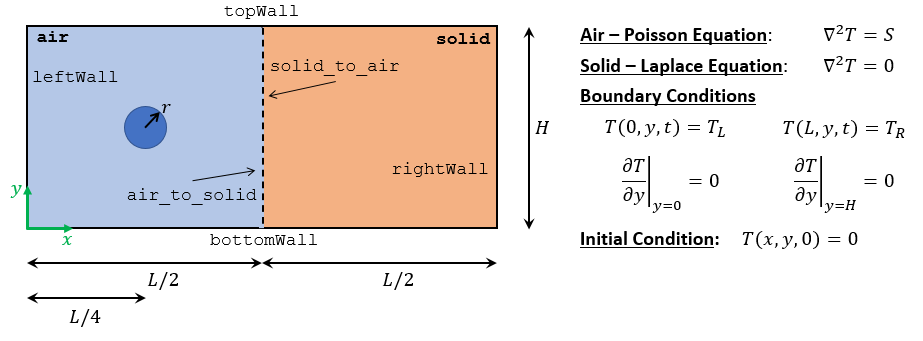
\includegraphics[width=0.9\textwidth]{source.png}
	\end{center}


	\item In the solver, the $S$ {\tt volScalarField} must be defined in the {\tt createFields.H}. 
	
	\begin{myframe}
	{\tt 
	Info<< "Calculating field S\textbackslash n" << endl;\\
	volScalarField S\\
	(\\
	\tab IOobject\\
	\tab (\\
	\tab \tab "S",\\
	\tab \tab runTime.timeName(),\\
	\tab \tab meshA,\\
	\tab \tab IOobject::MUST\_READ,\\
	\tab \tab IOobject::AUTO\_WRITE\\
	\tab ),\\
	\tab meshA\\
	);\\
	}
	\end{myframe}
	
	The Laplace equation for the air region must me modified into the Poisson equation as follows:
	
	\begin{myframe}
	{\tt 
        solve \\
		(\\
		\tab fvm::laplacian(Tair) - S\\
		);
	}
	\end{myframe}

	\newpage

	\item Run the case and evaluate the results.
	
	\begin{figure}[h]
		\centering
		\begin{subfigure}{\textwidth}
			\centering
			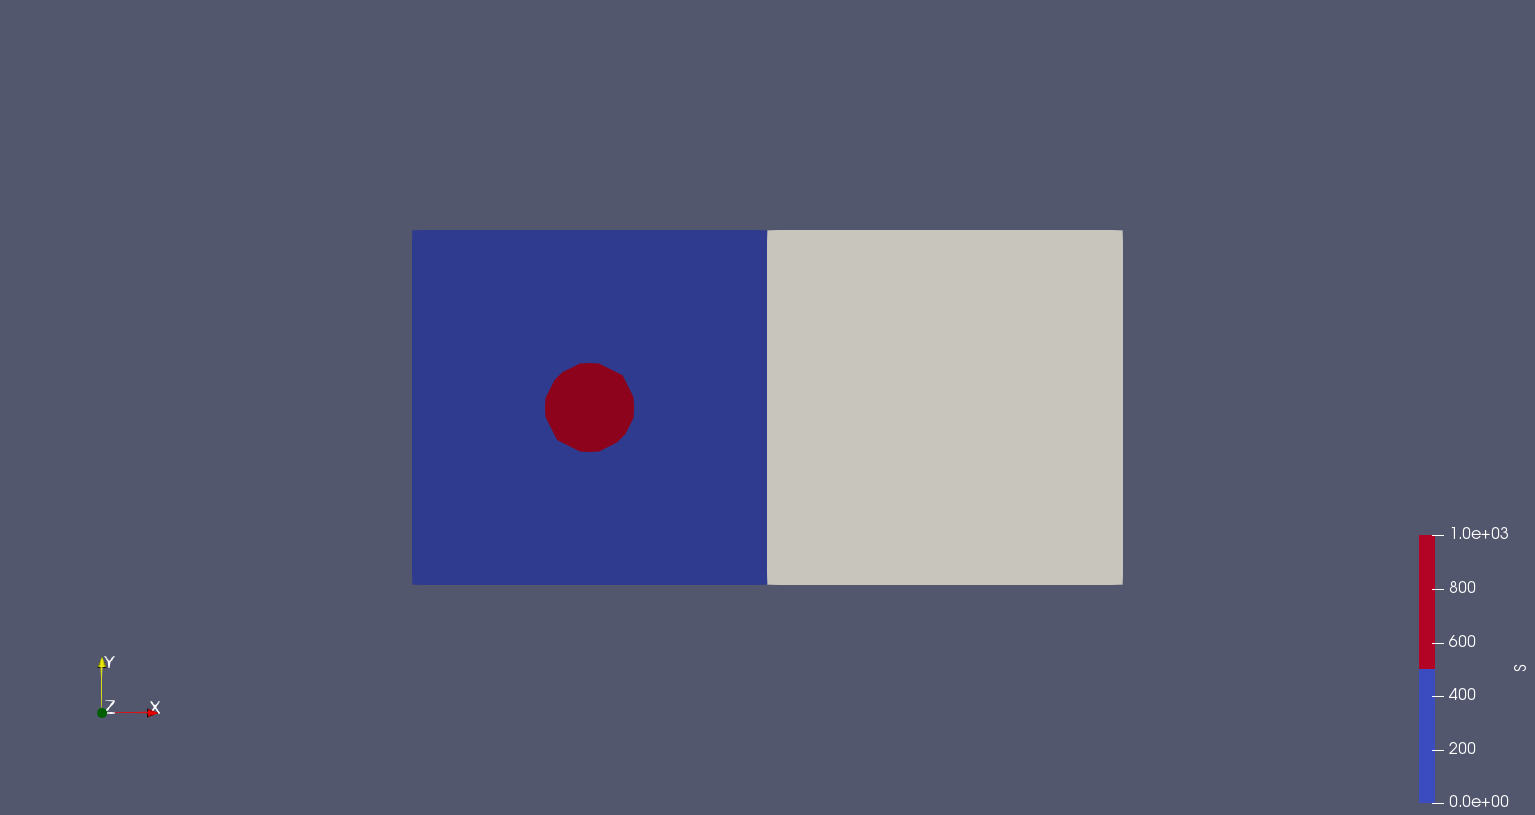
\includegraphics[width=0.9\textwidth]{S.png}
			\caption{Heat source}
		\end{subfigure}
		\begin{subfigure}{\textwidth}
			\centering
			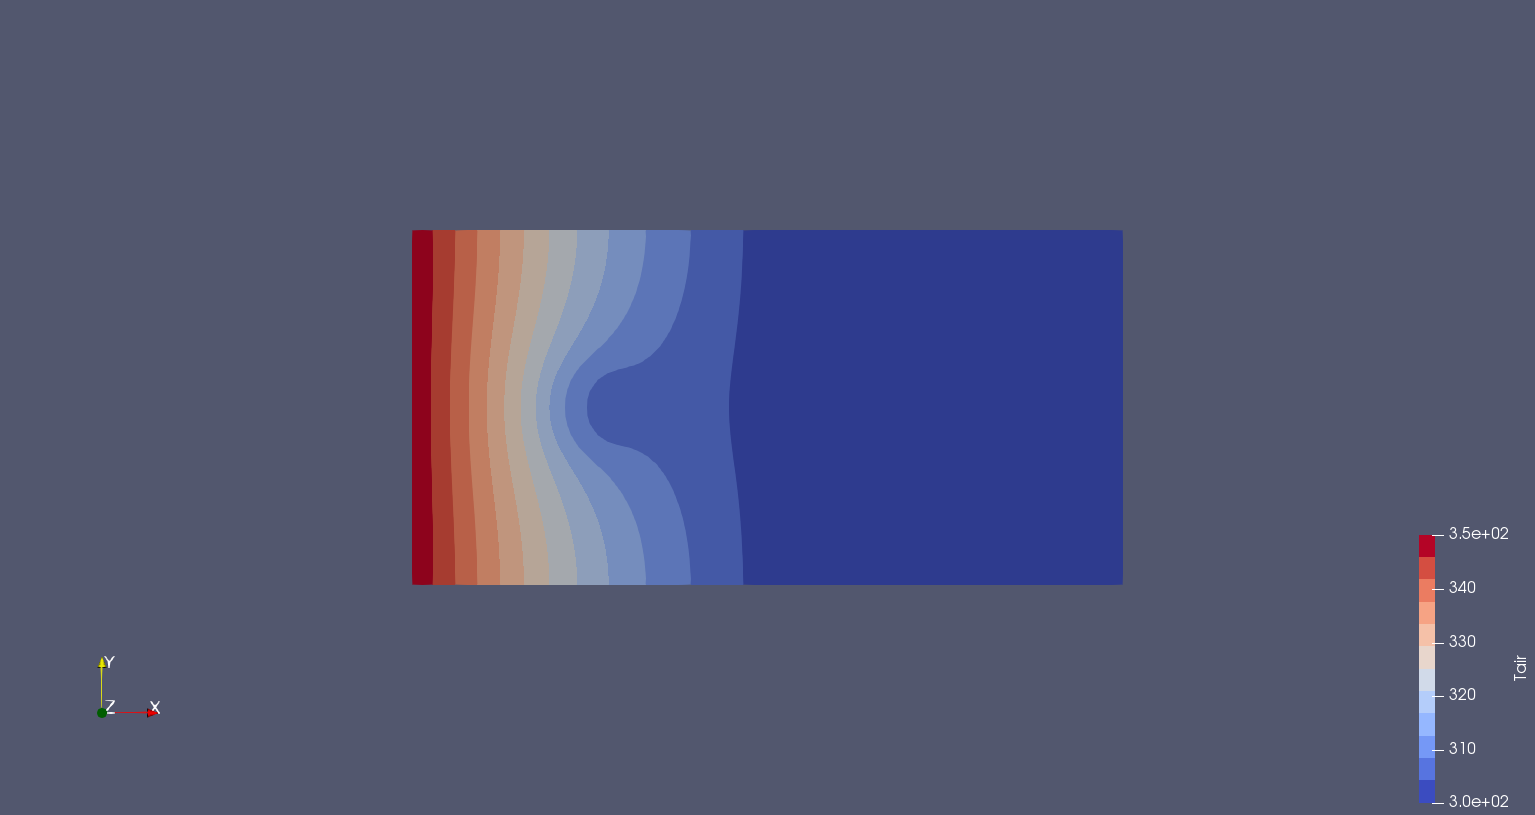
\includegraphics[width=0.9\textwidth]{T.png}
			\caption{Temperature}
		\end{subfigure}
	\end{figure}
	
	
\end{enumerate}


%	\begin{myframe}
%	{\tt 
%		
%		vertices\\
%		(\\
%		\tab (0 0 0)~~~~~// point 0\\
%		\tab (1 0 0)~~~~~// point 1\\
%		\tab (1 1 0)~~~~~// point 2\\
%		\tab (0 1 0)~~~~~// point 3\\
%		\tab (0 0 0.1)~~~// point 4\\
%		\tab (1 0 0.1)~~~// point 5\\
%		\tab (1 1 0.1)~~~// point 6\\
%		\tab (0 1 0.1)~~~// point 7\\
%		\tab (2 0 0)~~~~~// point 8\\
%		\tab (2 1 0)~~~~~// point 9\\
%		\tab (2 0 0.1)~~~// point 10\\
%		\tab (2 1 0.1)~~~// point 11\\
%		);\\
%		\\
%		blocks\\
%		(\\
%		\tab hex (0 1 2  3  4  5  6  7) air (20 20 1) simpleGrading (1 1 1)\\
%		\tab hex (1 8 9 2 5 10 11 6) solid (20 20 1) simpleGrading (1 1 1)\\
%		);
%	}
%	\end{myframe}










\end{document}